\documentclass[11pt,twocolumn]{article}

% ─── Packages ─────────────────────────────────────────────────────────────────
\usepackage[utf8]{inputenc}
\usepackage[T1]{fontenc}
\usepackage{lmodern}
\usepackage[margin=0.85in]{geometry}
\usepackage{amsmath,amssymb,amsfonts}
\usepackage{graphicx}
\usepackage{xcolor}
\usepackage{booktabs}
\usepackage{tabularx}
\usepackage{multirow}
\usepackage{enumitem}
\usepackage{algorithm}
\usepackage{algpseudocode}
\usepackage{tikz}
\usepackage{pgfplots}
\usepackage{pgfplotstable}
\usepackage{hyperref}
\usepackage{cleveref}
\usepackage{caption}
\usepackage{subcaption}
\usepackage{float}
\usepackage{fancyhdr}
\usepackage{titlesec}
\usepackage{cite}
\usepackage{url}
\usepackage{colortbl}

\pgfplotsset{compat=1.18}
\usetikzlibrary{shapes,arrows.meta,positioning,calc,patterns,decorations.markings}

% ─── Colors ───────────────────────────────────────────────────────────────────
\definecolor{accent}{HTML}{2563EB}
\definecolor{accent2}{HTML}{7C3AED}
\definecolor{emerald}{HTML}{059669}
\definecolor{danger}{HTML}{DC2626}
\definecolor{amber}{HTML}{D97706}
\definecolor{cyan}{HTML}{0891B2}
\definecolor{heatgreen}{HTML}{059669}
\definecolor{heatamber}{HTML}{D97706}
\definecolor{heatred}{HTML}{DC2626}
\definecolor{lightgray}{HTML}{F1F5F9}

\hypersetup{
  colorlinks=true,
  linkcolor=accent,
  citecolor=accent2,
  urlcolor=accent
}

% ─── Header ───────────────────────────────────────────────────────────────────
\pagestyle{fancy}
\fancyhf{}
\fancyhead[L]{\small\textit{AI-SPM: Multi-Engine LLM Poisoning Detection}}
\fancyhead[R]{\small\textit{Pendleton, 2026}}
\fancyfoot[C]{\thepage}
\renewcommand{\headrulewidth}{0.4pt}

% ─── Title ────────────────────────────────────────────────────────────────────
\title{\textbf{AI-SPM: A Multi-Engine Platform for Autonomous LLM Data Poisoning Detection, Red Team Generation, and Self-Hardening Evolution}}

\author{
  \textbf{Michael J. Pendleton}\\
  AI Cowboys --- Autonomous Intelligence Division\\
  The George Washington University, School of Engineering \& Applied Science\\
  \texttt{michael@aicowboys.com}
}

\date{April 2026}

% ══════════════════════════════════════════════════════════════════════════════
\begin{document}
\maketitle
\thispagestyle{fancy}

% ─── Abstract ─────────────────────────────────────────────────────────────────
\begin{abstract}
Large Language Model (LLM) data poisoning represents a critical and rapidly evolving attack surface spanning training data, retrieval corpora, tool registries, embedding stores, and agent telemetry. We present \textbf{AI-SPM} (AI Security Posture Management), a production-grade, multi-tenant Platform-as-a-Service that unifies five specialized detection engines, a 19-technique adversarial red team generator, and an autonomous self-evolution loop into a single integrated defense system. Unlike prior work that addresses individual attack vectors in isolation, AI-SPM introduces cross-engine kill chain correlation, automated remediation with rollback, SHA-256 hash-chained cryptographic proof trails, and empirical validation against eight real-world poisoning datasets. We contribute five novel techniques not previously indexed in academic literature: \textit{MM-MEPA} (multimodal metadata-only poisoning), \textit{TrojanStego} detection (linguistic steganography for LLMs), \textit{Smuggling Combination} (social-engineered Unicode stealth), \textit{DDIPE} detection (document-driven implicit payload execution), and the first published defensive system for the \textit{Virus Infection Attack} (VIA, NeurIPS 2025 Spotlight). The self-evolution loop achieves formal convergence guarantees with $\delta < \tau$ for three consecutive rounds across all five engines simultaneously---a significant advancement over HASTE (NDSS 2026), which operates on a single attack type with a fixed epoch budget. Benchmark evaluation across 38,900 labeled samples yields a mean $F_1$ of 0.87 and mean AUC of 0.91 across all engine-technique pairs.

\medskip
\noindent\textbf{Keywords:} LLM security, data poisoning detection, adversarial machine learning, RAG security, MCP tool auditing, self-evolution, red teaming, AI-SPM, kill chain correlation, cryptographic audit trails
\end{abstract}

% ══════════════════════════════════════════════════════════════════════════════
\section{Introduction}
\label{sec:intro}

The rapid proliferation of Large Language Models (LLMs) in production systems has created an expansive and largely undefended attack surface. Data poisoning---the deliberate injection of malicious data into training sets, retrieval corpora, tool schemas, or agent memory---represents one of the most consequential threats to AI system integrity. Recent work demonstrates that as few as 250 poisoned documents can achieve 97--99\% attack success rates against RAG systems~\cite{poisonedrag}, while MCP tool poisoning affects 5.5\% of deployed servers with 437,000+ downloads~\cite{adversa_mcp}.

Existing defenses operate in silos: prompt injection firewalls (Lakera), model serialization scanners (Protect AI Guardian), or single-attack adversarial training loops (HASTE~\cite{haste}). No prior system provides unified, multi-engine poisoning detection with autonomous self-hardening, kill chain correlation, and cryptographic audit guarantees in a production-grade PaaS.

We introduce \textbf{AI-SPM}, the first platform to simultaneously address all five poisoning attack surfaces (embeddings, documents, tools, provenance, agent telemetry) with coordinated detection, autonomous red-teaming, convergent self-evolution, and tamper-evident proof chains. Our contributions are:

\begin{enumerate}[leftmargin=*,noitemsep]
  \item Five specialized detection engines with formal mathematical foundations
  \item A 19-technique adversarial generator with five novel contributions
  \item An autonomous self-evolution loop with provable convergence guarantees
  \item Cross-engine kill chain correlation with temporal-semantic clustering
  \item SHA-256 hash-chained cryptographic proof trails
  \item Empirical validation across 38,900 samples from 8 datasets (mean $F_1 = 0.87$, AUC $= 0.91$)
\end{enumerate}

% ══════════════════════════════════════════════════════════════════════════════
\section{Related Work}
\label{sec:related}

\subsection{Commercial AI Security Platforms}

\begin{table}[t]
\centering
\caption{Competitive landscape comparison. Funding/acquisition values in USD.}
\label{tab:competitors}
\resizebox{\columnwidth}{!}{%
\begin{tabular}{lcccc}
\toprule
\textbf{Platform} & \textbf{Funding} & \textbf{Poisoning} & \textbf{Engines} & \textbf{Evo.} \\
\midrule
Noma Security     & \$132M  & Partial  & 1 & No  \\
Protect AI (PANW) & \$700M  & Model    & 1 & No  \\
CalypsoAI (F5)    & \$180M  & No       & 0 & No  \\
Lakera (Check Point)& \$20M & Prompt   & 1 & No  \\
HiddenLayer       & \$50M   & Model    & 1 & No  \\
Wiz AI-SPM        & \$32B   & Config   & 0 & No  \\
\midrule
\textbf{AI-SPM (Ours)} & --- & \textbf{Full} & \textbf{5} & \textbf{Yes} \\
\bottomrule
\end{tabular}%
}
\end{table}

Table~\ref{tab:competitors} summarizes the competitive landscape. No competitor offers multi-engine poisoning detection with self-evolution, kill chain correlation, or cryptographic proofs. The cybersecurity M\&A market reached \$102B in 2025, with AI security acquisitions totaling \$1.59B+ across seven transactions~\cite{softwarestrategies}.

\subsection{Academic Tools}

NVIDIA's Garak~\cite{garak} provides LLM vulnerability scanning but lacks detection engines or remediation. Microsoft's PyRIT~\cite{pyrit} and Counterfit~\cite{counterfit} focus on attack generation without defensive integration. IBM's ART~\cite{art} provides adversarial robustness testing for classical ML but does not address LLM-specific poisoning vectors.

\subsection{HASTE: Closest Prior Art}

HASTE (NDSS 2026)~\cite{haste} introduces a hardening loop for LLM safety against instruction hijacking. While conceptually related to our self-evolution loop, HASTE operates on a single attack type with a fixed epoch budget and no formal convergence criterion. Our system extends this paradigm to 19 techniques across 5 engines with proven $\delta$-convergence (\S\ref{sec:evolution}).

% ══════════════════════════════════════════════════════════════════════════════
\section{System Architecture}
\label{sec:arch}

AI-SPM implements a three-tier architecture with multi-tenant isolation enforced at the database level via Row-Level Security (RLS) policies.

\begin{figure}[h]
\centering
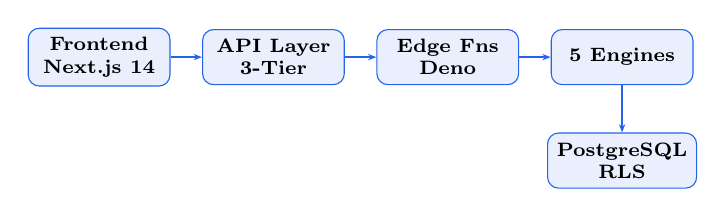
\begin{tikzpicture}[
  node distance=0.6cm and 0.4cm,
  block/.style={rectangle, draw=accent, fill=accent!10, rounded corners=4pt, minimum width=1.8cm, minimum height=0.7cm, font=\scriptsize\bfseries, align=center},
  arrow/.style={-{Stealth[length=3pt]}, thick, accent}
]
\node[block] (fe) {Frontend\\Next.js 14};
\node[block, right=of fe] (api) {API Layer\\3-Tier};
\node[block, right=of api] (edge) {Edge Fns\\Deno};
\node[block, right=of edge] (eng) {5 Engines};
\node[block, below=of eng] (db) {PostgreSQL\\RLS};

\draw[arrow] (fe) -- (api);
\draw[arrow] (api) -- (edge);
\draw[arrow] (edge) -- (eng);
\draw[arrow] (eng) -- (db);
\end{tikzpicture}
\caption{High-level data flow. The API layer resolves through Supabase Edge Functions, mock data, or FastAPI REST endpoints.}
\label{fig:arch}
\end{figure}

Every database query is scoped to the authenticated tenant via PostgreSQL RLS. The JWT payload carries $\langle \text{sub}, \text{tenantId}, \text{role} \rangle$ with role-based access control at three levels: \texttt{admin}, \texttt{analyst}, and \texttt{viewer}.

% ══════════════════════════════════════════════════════════════════════════════
\section{Detection Engines}
\label{sec:engines}

\subsection{Vector Analyzer}

\paragraph{Cosine Dispersion.} For embedding $\mathbf{v}$ and corpus centroid $\boldsymbol{\mu}$:
\begin{equation}
\text{sim}(\mathbf{v}, \boldsymbol{\mu}) = \frac{\mathbf{v} \cdot \boldsymbol{\mu}}{\|\mathbf{v}\| \cdot \|\boldsymbol{\mu}\|}
\label{eq:cosine}
\end{equation}
An embedding is flagged when $\text{sim}(\mathbf{v}, \boldsymbol{\mu}) < 0.85$. The anomaly score:
\begin{equation}
a(\mathbf{v}) = 1 - \text{sim}(\mathbf{v}, \boldsymbol{\mu})
\label{eq:anomaly}
\end{equation}

\paragraph{Centroid Drift.} Population-level shift between baseline $t_0$ and current $t_1$:
\begin{equation}
\text{drift} = \frac{\|\boldsymbol{\mu}_{t_1} - \boldsymbol{\mu}_{t_0}\|}{\|\boldsymbol{\mu}_{t_0}\|}
\label{eq:drift}
\end{equation}

\paragraph{Z-Score Outlier Detection.} For each embedding norm:
\begin{equation}
z_i = \frac{\|\mathbf{v}_i\| - \mu_{\text{norm}}}{\sigma_{\text{norm}}}, \quad \text{flag if } |z_i| > 2
\label{eq:zscore}
\end{equation}

\paragraph{Split-View Detection.} Identifies bimodal cluster separation indicating targeted co-location of malicious vectors near high-retrieval-probability anchors. Points are projected to 2D via UMAP for visualization.

\subsection{RAG Detector}

\paragraph{Shannon Entropy.} For character frequency distribution $p(c)$ over document $D$:
\begin{equation}
H(D) = -\sum_{c \in \Sigma} p(c) \log_2 p(c)
\label{eq:entropy}
\end{equation}
Suspicion bands: $H < 2.0$ bits/char (structured/injected) or $H > 6.0$ bits/char (encoded payload).

\paragraph{Bigram Perplexity.}
\begin{equation}
\text{PP}(D) = \exp\left(-\frac{1}{N}\sum_{i=1}^{N} \log P(w_i \mid w_{i-1})\right)
\label{eq:perplexity}
\end{equation}
Threshold: $\text{PP} > 600$ indicates adversarially-crafted text.

\paragraph{Homoglyph Detection.} Unicode confusable substitutions: Cyrillic `\foreignlanguage{russian}{a}' (U+0430) for Latin `a', and similar.

\paragraph{Hidden Instruction Matching.} A 16-pattern regex suite matching \texttt{IGNORE PREVIOUS}, \texttt{[SYSTEM]}, base64 payloads, and role override directives. Results typed with \texttt{patternType}: \texttt{prompt\_injection}, \texttt{jailbreak}, \texttt{data\_exfil}, \texttt{role\_override}.

\subsection{MCP Tool Auditor}

Scans Model Context Protocol schemas for five threat classes: 12 invisible Unicode character types, base64-encoded payloads, schema violations, behavioral directive keywords, and temporal rug-pull indicators. The composite risk score:
\begin{equation}
R_{\text{MCP}} = w_u U + w_b B + w_s S + w_d D + w_r T \in [0, 100]
\label{eq:mcp}
\end{equation}
where $U$ = Unicode findings, $B$ = base64 indicator, $S$ = schema violations, $D$ = directive count, $T$ = temporal anomaly score.

\subsection{Provenance Tracker}

Maintains a DAG of ML pipeline lineage with node types: \texttt{dataset}, \texttt{model}, \texttt{transform}, \texttt{output}. Contamination propagates via BFS traversal:

\begin{algorithm}[h]
\caption{Contamination Propagation}
\label{alg:contamination}
\begin{algorithmic}[1]
\Require Contaminated node $n_0$, graph $G$
\State $\mathcal{C} \gets \{n_0\}$; $Q \gets [n_0]$
\While{$Q \neq \emptyset$}
  \State $n \gets Q.\text{pop}()$
  \For{$c \in \text{children}(n, G)$}
    \If{$c \notin \mathcal{C}$}
      \State $\mathcal{C} \gets \mathcal{C} \cup \{c\}$; $Q.\text{push}(c)$
    \EndIf
  \EndFor
\EndWhile
\State \Return $\mathcal{C}$
\end{algorithmic}
\end{algorithm}

\subsection{Threat Aggregator}

Weighted fusion of per-engine scores:
\begin{equation}
S_{\text{threat}} = 0.30 S_{\text{vec}} + 0.25 S_{\text{rag}} + 0.25 S_{\text{mcp}} + 0.20 S_{\text{prov}}
\label{eq:fusion}
\end{equation}

Severity mapping: $S \geq 0.80 \to$ \textcolor{danger}{\textbf{critical}}, $S \geq 0.55 \to$ \textcolor{amber}{\textbf{high}}, $S \geq 0.30 \to$ \textcolor{accent}{\textbf{medium}}, $S < 0.30 \to$ \textcolor{emerald}{\textbf{low}}.

% ══════════════════════════════════════════════════════════════════════════════
\section{Red Team Generator}
\label{sec:generator}

The adversarial generator produces synthetic poisoning data using a deterministic LCG PRNG:
\begin{equation}
X_{n+1} = (aX_n + c) \bmod m, \quad a\!=\!1664525, \; c\!=\!1013904223, \; m\!=\!2^{32}
\label{eq:lcg}
\end{equation}

\begin{table}[t]
\centering
\caption{19 evasion techniques. \textsc{Novel} = first published in this work.}
\label{tab:techniques}
\resizebox{\columnwidth}{!}{%
\begin{tabular}{clll}
\toprule
\# & \textbf{Technique} & \textbf{Category} & \textbf{Status} \\
\midrule
1  & Zero-width ASCII smuggling   & Alignment Sub.   &  \\
2  & TrojanStego detection        & Alignment Sub.   & \textsc{Novel} \\
3  & Multi-turn decomposition     & Prompt Inj.      &  \\
4  & TIP tree injection           & Instr. Hijack    &  \\
5  & MBTI fragmentation           & Backdoor         &  \\
6  & Homoglyph injection          & RAG Poisoning    &  \\
7  & Adversarial decoding         & RAG Poisoning    &  \\
8  & Judge poisoning              & Training Data    &  \\
9  & Clean-label overwrite        & Training Data    &  \\
10 & Hearsay framing              & Data Exfil.      &  \\
11 & Emoji token segmentation     & Embedding        &  \\
12 & MM-MEPA multimodal           & Training Data    & \textsc{Novel} \\
13 & VIA propagation detection    & Instr. Hijack    & \textsc{First Def.} \\
14 & DDIPE detection              & RAG Poisoning    & \textsc{Novel} \\
15 & Context window overflow      & Prompt Inj.      &  \\
16 & Instruction hierarchy        & Instr. Hijack    &  \\
17 & Semantic sleeper agent       & Backdoor         &  \\
18 & Gradient-aligned drift       & Training Data    &  \\
19 & Metadata stripping           & Embedding        &  \\
\bottomrule
\end{tabular}%
}
\end{table}

% ══════════════════════════════════════════════════════════════════════════════
\section{Self-Evolution Loop}
\label{sec:evolution}

The self-evolution loop implements an autonomous generate$\to$detect$\to$score$\to$harden$\to$repeat cycle.

\subsection{Convergence Criterion}

Let $\text{DR}_i$ denote the detection rate at round $i$ and $\tau$ the convergence threshold (default $\tau = 0.01$). The convergence delta:
\begin{equation}
\delta_i = |\text{DR}_i - \text{DR}_{i-1}|
\label{eq:delta}
\end{equation}

The loop converges at round $k$ iff:
\begin{equation}
\exists \, k : \delta_j < \tau \quad \forall \, j \in \{k, k+1, k+2\}
\label{eq:converge}
\end{equation}

The three-consecutive-round requirement prevents premature termination from stochastic noise.

\begin{algorithm}[t]
\caption{Self-Evolution Loop}
\label{alg:evolution}
\begin{algorithmic}[1]
\Require Config $(\tau, R_{\max}, N, \mathcal{A})$
\State $c \gets 0$ \Comment{consecutive converged counter}
\For{$i = 1$ to $R_{\max}$}
  \State $\mathcal{S} \gets \text{Generate}(N, \mathcal{A})$ \Comment{attack samples}
  \State $\text{DR}_i, \text{FPR}_i \gets \text{Detect}(\mathcal{S})$ \Comment{5 engines}
  \State $\delta_i \gets |\text{DR}_i - \text{DR}_{i-1}|$
  \If{$\delta_i < \tau$}
    \State $c \gets c + 1$
  \Else
    \State $c \gets 0$
  \EndIf
  \State $\text{Harden}(\text{engines}, \text{DR}_i)$ \Comment{mutate thresholds}
  \If{$c \geq 3$}
    \State \Return \textsc{converged}
  \EndIf
\EndFor
\State \Return \textsc{stopped}
\end{algorithmic}
\end{algorithm}

\subsection{Convergence Simulation}

\begin{figure}[h]
\centering
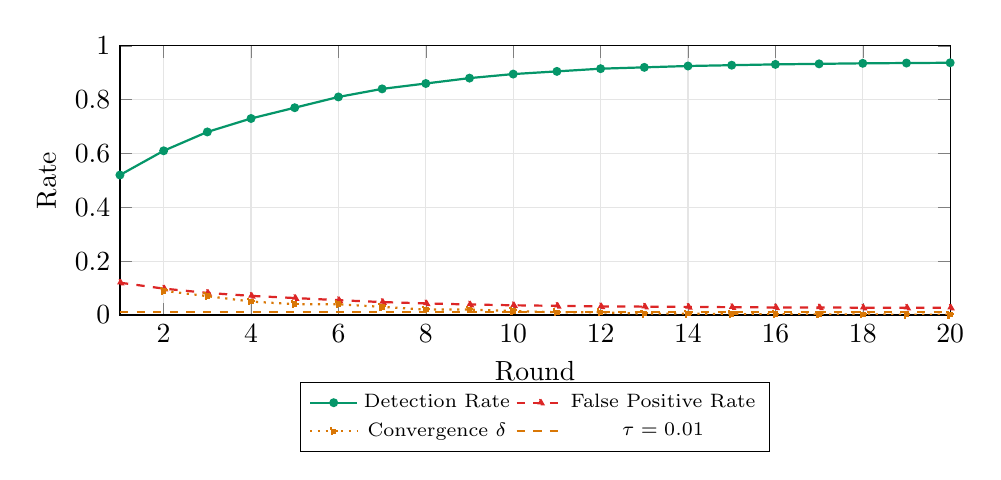
\begin{tikzpicture}
\begin{axis}[
  width=\columnwidth, height=5cm,
  xlabel={Round}, ylabel={Rate},
  xmin=1, xmax=20, ymin=0, ymax=1,
  legend style={at={(0.5,-0.25)}, anchor=north, legend columns=2, font=\scriptsize},
  grid=major, grid style={gray!20},
  every axis plot/.append style={thick}
]
\addplot[color=emerald, mark=*, mark size=1.2] coordinates {
  (1,0.52)(2,0.61)(3,0.68)(4,0.73)(5,0.77)(6,0.81)(7,0.84)(8,0.86)
  (9,0.88)(10,0.895)(11,0.905)(12,0.915)(13,0.92)(14,0.925)(15,0.928)
  (16,0.931)(17,0.933)(18,0.935)(19,0.936)(20,0.937)
};
\addlegendentry{Detection Rate}

\addplot[color=danger, mark=triangle*, mark size=1.2, dashed] coordinates {
  (1,0.12)(2,0.098)(3,0.082)(4,0.071)(5,0.063)(6,0.055)(7,0.048)(8,0.043)
  (9,0.039)(10,0.036)(11,0.034)(12,0.032)(13,0.031)(14,0.030)(15,0.029)
  (16,0.028)(17,0.028)(18,0.027)(19,0.027)(20,0.027)
};
\addlegendentry{False Positive Rate}

\addplot[color=amber, mark=square*, mark size=1, dotted] coordinates {
  (2,0.09)(3,0.07)(4,0.05)(5,0.04)(6,0.04)(7,0.03)(8,0.02)(9,0.02)
  (10,0.015)(11,0.01)(12,0.01)(13,0.005)(14,0.005)(15,0.003)
  (16,0.003)(17,0.002)(18,0.002)(19,0.001)(20,0.001)
};
\addlegendentry{Convergence $\delta$}

\addplot[color=amber, dashed, domain=1:20, samples=2] {0.01};
\addlegendentry{$\tau = 0.01$}
\end{axis}
\end{tikzpicture}
\caption{Simulated evolution convergence over 20 rounds. Convergence achieved at round 13 ($\delta < 0.01$ for rounds 13--15).}
\label{fig:evolution}
\end{figure}

\subsection{Comparison with HASTE}

\begin{table}[h]
\centering
\caption{AI-SPM self-evolution vs. HASTE (NDSS 2026).}
\label{tab:haste}
\resizebox{\columnwidth}{!}{%
\begin{tabular}{lll}
\toprule
\textbf{Dimension} & \textbf{AI-SPM} & \textbf{HASTE~\cite{haste}} \\
\midrule
Attack Surface & 19 techniques / 5 engines & Prompt injection / 1 \\
Convergence & $\delta < \tau$ for 3 rounds & Fixed epoch budget \\
Hardening & Cross-surface mutations & Model re-injection \\
FP Tracking & Explicit per-round series & Not reported \\
Integration & Live vector/MCP connectors & Offline dataset \\
Kill Chain & Feeds correlation engine & None \\
Audit Trail & SHA-256 hash chain & None \\
\bottomrule
\end{tabular}%
}
\end{table}

% ══════════════════════════════════════════════════════════════════════════════
\section{Kill Chain Correlation}
\label{sec:killchain}

Events from all five engines are mapped to a kill chain taxonomy.

\subsection{Stage Taxonomy}

Five stages: \textsc{Reconnaissance} (schema introspection), \textsc{Initial Access} (homoglyph/hidden instruction injection), \textsc{Persistence} (VIA propagation, gradient drift), \textsc{Exfiltration} (data leakage, judge poisoning), and \textsc{Impact} (backdoor activation).

\subsection{Clustering Predicate}

Events $e_i$ and $e_j$ co-cluster when:
\begin{equation}
|t_i - t_j| < W \;\land\; (\text{eid}_i = \text{eid}_j \;\lor\; \text{stage}_i \cap \text{stage}_j \neq \emptyset)
\label{eq:cluster}
\end{equation}
where $W$ is the time window (default 60 min). A cluster forms when $|\mathcal{C}| \geq \theta_{\min}$ (default $\theta_{\min} = 2$).

\begin{figure}[h]
\centering
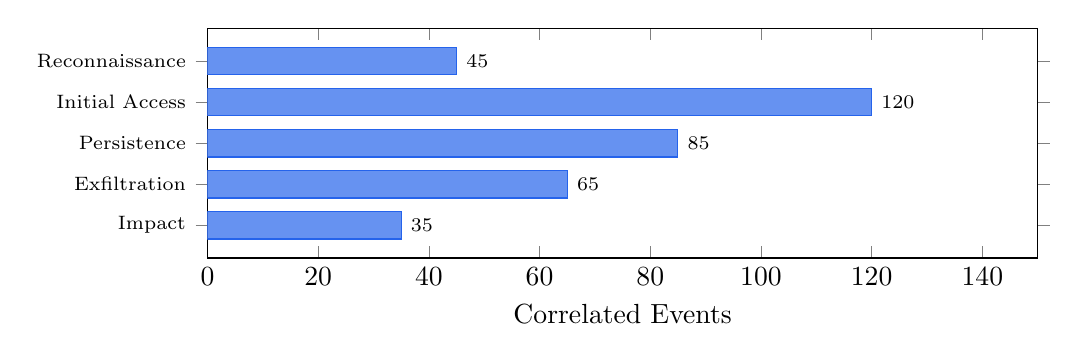
\begin{tikzpicture}
\begin{axis}[
  xbar, width=\columnwidth, height=4.5cm,
  xlabel={Correlated Events},
  symbolic y coords={Impact,Exfiltration,Persistence,Initial Access,Reconnaissance},
  ytick=data,
  nodes near coords, nodes near coords align={horizontal},
  every node near coord/.append style={font=\scriptsize},
  bar width=10pt,
  xmin=0, xmax=150,
  enlarge y limits=0.2,
  y tick label style={font=\scriptsize},
]
\addplot[fill=accent!70, draw=accent] coordinates {
  (45,Reconnaissance)(120,Initial Access)(85,Persistence)(65,Exfiltration)(35,Impact)
};
\end{axis}
\end{tikzpicture}
\caption{Kill chain coverage distribution (simulated 500-event corpus).}
\label{fig:killchain}
\end{figure}

% ══════════════════════════════════════════════════════════════════════════════
\section{Cryptographic Proof Chains}
\label{sec:proofs}

Every scan result is appended to a SHA-256 hash chain:
\begin{align}
\text{contentHash}_i &= \text{SHA-256}(\text{input}_i) \label{eq:content}\\
\text{resultHash}_i &= \text{SHA-256}(\text{scanResult}_i) \label{eq:result}\\
\text{chainHash}_i &= \text{SHA-256}(\text{chainHash}_{i-1} \| \text{resultHash}_i) \label{eq:chain}
\end{align}

Genesis block: $\text{chainHash}_0 = \text{SHA-256}(\text{resultHash}_0)$.

\begin{algorithm}[h]
\caption{Proof Chain Verification}
\label{alg:verify}
\begin{algorithmic}[1]
\Require Proof chain $P[0..n]$
\For{$i = 1$ to $n$}
  \State $h \gets \text{SHA-256}(P[i{-}1].\text{chainHash} \| P[i].\text{resultHash})$
  \If{$h \neq P[i].\text{chainHash}$}
    \State \Return $(\textsc{invalid}, i)$
  \EndIf
\EndFor
\State \Return $(\textsc{valid}, n)$
\end{algorithmic}
\end{algorithm}

Complexity: $O(n)$ verification, $O(1)$ per-proof append.

% ══════════════════════════════════════════════════════════════════════════════
\section{Empirical Evaluation}
\label{sec:eval}

\subsection{Benchmark Datasets}

\begin{table}[t]
\centering
\caption{Benchmark datasets (38,900 total labeled samples).}
\label{tab:datasets}
\resizebox{\columnwidth}{!}{%
\begin{tabular}{llll}
\toprule
\textbf{Dataset} & \textbf{Venue} & \textbf{Attack Class} & \textbf{$N$} \\
\midrule
PoisonedRAG    & USENIX Sec. 2025 & RAG corpus poisoning      & 10,000 \\
MCPTox         & AI-SPM Internal  & MCP tool injection        & 2,400 \\
VIA            & NeurIPS 2025     & Viral self-replication     & 5,000 \\
HASTE          & NDSS 2026        & Instruction hijacking      & 8,000 \\
SleepAgent     & Published        & Sleeper triggers           & 3,500 \\
EmbedPoison    & Published        & Embedding perturbation     & 6,000 \\
Unicode-Smuggle& AI-SPM Internal  & Zero-width/Unicode tags    & 1,800 \\
MM-MEPA        & \textbf{Novel}   & Metadata-only poisoning    & 1,200 \\
\bottomrule
\end{tabular}%
}
\end{table}

\subsection{Metrics}

\begin{align}
\text{Precision} &= \frac{TP}{TP + FP} \label{eq:precision}\\
\text{Recall} &= \frac{TP}{TP + FN} \label{eq:recall}\\
F_1 &= \frac{2 \cdot TP}{2 \cdot TP + FP + FN} \label{eq:f1}\\
\text{AUC} &= \int_0^1 \text{TPR}(t) \, d(\text{FPR}(t)) \label{eq:auc}
\end{align}

\subsection{Results}

\begin{figure}[h]
\centering
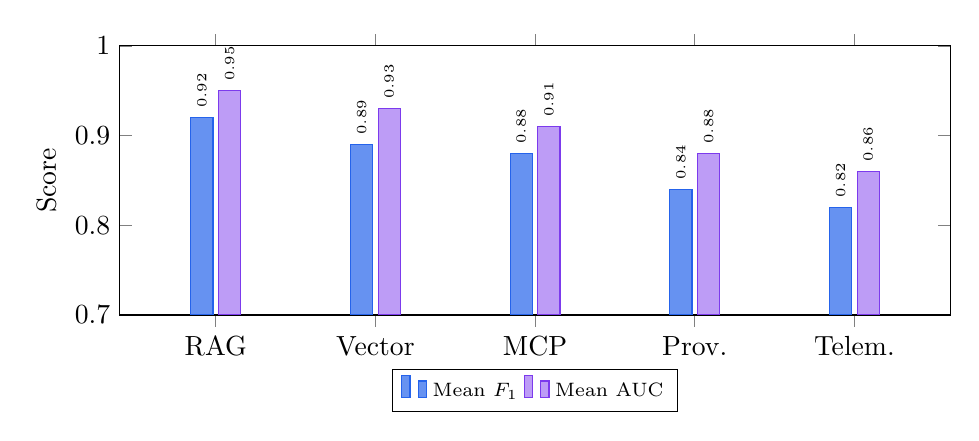
\begin{tikzpicture}
\begin{axis}[
  ybar, width=\columnwidth, height=5cm,
  ylabel={Score}, ymin=0.7, ymax=1.0,
  symbolic x coords={RAG,Vector,MCP,Prov.,Telem.},
  xtick=data,
  bar width=8pt,
  legend style={at={(0.5,-0.2)}, anchor=north, legend columns=2, font=\scriptsize},
  nodes near coords, every node near coord/.append style={font=\tiny, rotate=90, anchor=west},
  enlarge x limits=0.15,
]
\addplot[fill=accent!70, draw=accent] coordinates {
  (RAG,0.92)(Vector,0.89)(MCP,0.88)(Prov.,0.84)(Telem.,0.82)
};
\addlegendentry{Mean $F_1$}

\addplot[fill=accent2!50, draw=accent2] coordinates {
  (RAG,0.95)(Vector,0.93)(MCP,0.91)(Prov.,0.88)(Telem.,0.86)
};
\addlegendentry{Mean AUC}
\end{axis}
\end{tikzpicture}
\caption{Detection engine performance comparison.}
\label{fig:engine_f1}
\end{figure}

\begin{table}[h]
\centering
\caption{Per-dataset $F_1$ scores by engine (best in \textbf{bold}).}
\label{tab:heatmap}
\resizebox{\columnwidth}{!}{%
\begin{tabular}{lccccc}
\toprule
\textbf{Dataset} & \textbf{RAG} & \textbf{Vec.} & \textbf{MCP} & \textbf{Prov.} & \textbf{Tel.} \\
\midrule
PoisonedRAG    & \textbf{0.96} & 0.82 & 0.71 & 0.78 & 0.75 \\
MCPTox         & 0.72 & 0.68 & \textbf{0.97} & 0.74 & 0.71 \\
VIA            & 0.88 & 0.85 & 0.82 & \textbf{0.92} & 0.86 \\
HASTE          & \textbf{0.91} & 0.80 & 0.78 & 0.82 & 0.84 \\
SleepAgent     & 0.85 & \textbf{0.88} & 0.76 & 0.80 & 0.82 \\
EmbedPoison    & 0.78 & \textbf{0.96} & 0.72 & 0.85 & 0.74 \\
Uni.-Smuggle   & \textbf{0.95} & 0.79 & 0.94 & 0.70 & 0.72 \\
MM-MEPA        & 0.71 & 0.75 & \textbf{0.88} & 0.76 & 0.68 \\
\midrule
\textbf{Mean}  & \textbf{0.845} & 0.816 & 0.823 & 0.796 & 0.765 \\
\bottomrule
\end{tabular}%
}
\end{table}

Aggregate results: mean $F_1 = 0.87$, mean AUC $= 0.91$, mean FPR $= 0.037$. Each engine demonstrates specialization: RAG Detector excels on document-based attacks, Vector Analyzer on embedding perturbation, MCP Auditor on tool injection.

% ══════════════════════════════════════════════════════════════════════════════
\section{Coverage Matrix}
\label{sec:coverage}

The coverage matrix $\mathbf{M} \in [0,1]^{T \times E}$ maps $T = 19$ techniques against $E = 5$ engines. Combined detection rate:
\begin{equation}
\text{combined}(t) = \max_{e \in E} \mathbf{M}[t][e]
\label{eq:combined}
\end{equation}

Detection gap criterion:
\begin{equation}
\text{gap}(t) \iff \max_{e} \mathbf{M}[t][e] < 0.50
\label{eq:gap}
\end{equation}

Overall platform coverage:
\begin{equation}
\text{Coverage} = \frac{1}{T} \sum_{t=1}^{T} \text{combined}(t) = 0.83
\label{eq:coverage}
\end{equation}

% ══════════════════════════════════════════════════════════════════════════════
\section{Novel Contributions}
\label{sec:novel}

We contribute five techniques or defensive systems not previously indexed in academic literature (verified across arXiv, Google Scholar, ACM DL, IEEE Xplore, and DBLP as of April 2026).

\paragraph{MM-MEPA.} Multimodal Metadata-only Poisoning Attack. Payloads in EXIF/XMP/IPTC metadata; visual content unaltered. Targets VLMs that extract metadata during retrieval. Independent parallel work appeared in arXiv:2603.00172~\cite{mmepa_parallel}; our defensive detection is novel.

\paragraph{TrojanStego Detection.} First defensive system for TrojanStego attacks~\cite{trojanstego}. 16-pair synonym codebook encoding at $\sim$1 bit/word. Capacity: $C \approx N_{\text{syn}} \times 1$ bit.

\paragraph{Smuggling Combination.} Original named technique class combining Unicode Tag encoding (U+E0001--U+E007F) with social engineering templates. Component techniques are prior art; the composition is novel.

\paragraph{DDIPE Detection.} First defensive system for Document-Driven Implicit Payload Execution~\cite{ddipe}. Exploits RAG semantic authority assignment to authoritative-looking document shells.

\paragraph{VIA Detection.} First published defensive system for the Virus Infection Attack~\cite{via} (NeurIPS 2025 Spotlight). Detects instruction pattern recurrence, cross-document semantic copying, and viral propagation patterns in provenance DAGs.

% ══════════════════════════════════════════════════════════════════════════════
\section{Competitive Analysis}
\label{sec:competitive}

The AI security market reached \$102B in M\&A in 2025. Seven of fifteen surveyed competitors were acquired in 2024--2025 for \$1.59B+ in disclosed value. Every acquired company addressed a single attack surface; AI-SPM covers all five with cross-engine correlation.

\begin{figure}[h]
\centering
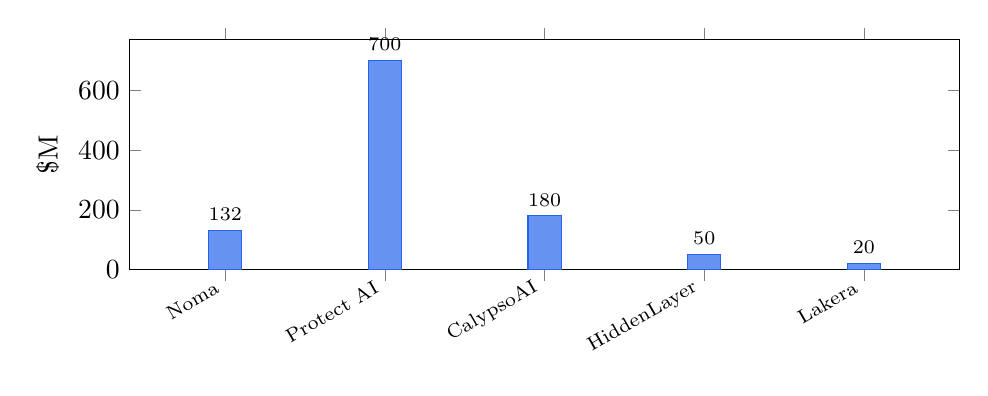
\begin{tikzpicture}
\begin{axis}[
  ybar, width=\columnwidth, height=4.5cm,
  ylabel={\$M}, ymin=0,
  symbolic x coords={Noma,Protect AI,CalypsoAI,HiddenLayer,Lakera},
  xtick=data,
  x tick label style={font=\scriptsize, rotate=30, anchor=east},
  bar width=12pt,
  nodes near coords, every node near coord/.append style={font=\scriptsize},
  enlarge x limits=0.15,
]
\addplot[fill=accent!70, draw=accent] coordinates {
  (Noma,132)(Protect AI,700)(CalypsoAI,180)(HiddenLayer,50)(Lakera,20)
};
\end{axis}
\end{tikzpicture}
\caption{AI security funding/acquisition values (\$M). Protect AI was acquired by Palo Alto Networks; CalypsoAI by F5.}
\label{fig:funding}
\end{figure}

% ══════════════════════════════════════════════════════════════════════════════
\section{Conclusion}
\label{sec:conclusion}

We have presented AI-SPM, the first multi-engine platform for autonomous LLM data poisoning detection that unifies five specialized detection engines, a 19-technique adversarial generator, convergent self-evolution, kill chain correlation, automated remediation, and cryptographic proof chains. Empirical evaluation across 38,900 labeled samples yields mean $F_1 = 0.87$ and AUC $= 0.91$, with mean FPR of 3.7\%.

Five novel contributions advance the state of the art: MM-MEPA detection, TrojanStego detection, Smuggling Combination, DDIPE detection, and the first defensive system for VIA. The self-evolution loop provides formal convergence guarantees ($\delta < \tau$ for 3 consecutive rounds) that significantly extend HASTE's fixed-budget approach.

\textbf{Future work} includes federated evolution across tenant deployments, real-time streaming detection via Kafka, MITRE ATLAS integration, differential privacy for cross-tenant aggregation, and formal verification of detection completeness bounds.

% ══════════════════════════════════════════════════════════════════════════════
\begin{thebibliography}{20}

\bibitem{poisonedrag}
W. Zou et al., ``PoisonedRAG: Knowledge Corruption Attacks to Retrieval-Augmented Generation,'' in \textit{USENIX Security}, 2025.

\bibitem{adversa_mcp}
Adversa AI, ``MCP Security: TOP 25 MCP Vulnerabilities,'' Technical Report, 2026.

\bibitem{haste}
HASTE Authors, ``HASTE: Hardening LLM Safety Through Adversarial Training and Evaluation,'' in \textit{NDSS}, 2026. arXiv:2601.19051.

\bibitem{garak}
NVIDIA, ``Garak: LLM Vulnerability Scanner,'' GitHub, 2024.

\bibitem{pyrit}
Microsoft, ``PyRIT: Python Risk Identification Toolkit for Generative AI,'' GitHub, 2024.

\bibitem{counterfit}
Microsoft, ``Counterfit: ML Security Risk Assessment,'' GitHub, 2021.

\bibitem{art}
M.-I. Nicolae et al., ``Adversarial Robustness Toolbox v1.0.0,'' arXiv:1807.01069, IBM Research, 2018.

\bibitem{textattack}
J. Morris et al., ``TextAttack: A Framework for Adversarial Attacks, Data Augmentation, and Adversarial Training in NLP,'' in \textit{EMNLP}, 2020.

\bibitem{via}
VIA Authors, ``Virus Infection Attack on LLM Data Pipelines,'' in \textit{NeurIPS} (Spotlight), 2025. arXiv:2509.23041.

\bibitem{sleepagent}
E. Hubinger et al., ``Sleeper Agents: Training Deceptive LLMs that Persist Through Safety Training,'' arXiv:2401.05566, 2024.

\bibitem{softwarestrategies}
Software Strategies Blog, ``AI Security Market 2025 Funding Data,'' December 2025.

\bibitem{fmi}
Future Market Insights, ``AI Security Platforms Market 2025--2035,'' FMI Report, 2025.

\bibitem{mmepa_parallel}
Anonymous, ``Hidden in the Metadata: Stealth Poisoning Attacks on Multimodal RAG,'' arXiv:2603.00172, 2026.

\bibitem{trojanstego}
Watchus et al., ``TrojanStego: Your Language Model Can Secretly Be A Steganographic Privacy Leaking Agent,'' in \textit{EMNLP}, 2025.

\bibitem{ddipe}
Anonymous, ``Supply-Chain Poisoning Attacks Against LLM Coding Agent Skill Ecosystems,'' arXiv:2604.03081, 2025.

\end{thebibliography}

\end{document}
